\section{Camera}
The mathematical form of the projection:
\[
	p_{\-{img}}
	=
	M_{\-{obj}2\-{img}}\cdot p_{\-{obj}}
	=
	M_{\-{cam}2\-{img}}M_{\-{world}2\-{cam}}M_{\-{obj}2\-{world}}\cdot p_{\-{obj}}
\]
\subsection{Camera to Film}
\subsubsection{Modeling the Pinhole Camera}
\[
	P(x,y,z)=\mqty(\flatfrac{hx}{z} & \flatfrac{hy}{z} & h)
.\]
Condsider homogeneous coordinates:
\[
	\mqty(
	1 & 0 & 0 & 0 \\
	0 & 1 & 0 & 0 \\
	0 & 0 & 1 & 0 \\
	0 & 0 & \*{1} & \*{0} \\
	)
	\mqty(x\\y\\z\\1)
	\qor
	\mqty(
	h & 0 & 0 & a \\
	0 & h & 0 & b \\
	0 & 0 & 1 & 0 \\
	0 & 0 & \*{1} & \*{0} \\
	)
	\mqty(x\\y\\z\\1)
.\]
\subsubsection{Viewing Frustrum}
\begin{itemize}
	\item Idea: transform viewing frustrum to an orthographic bounding box
	\item Instead of projecting everything to the plane at fixed depth, project to a cube first
	\item Clip anything thatʼs not within $-1\to 1$
\end{itemize}
\[
	\mqty(x'\\y'\\z'\\w')=
    \mqty(\displaystyle
	\flatfrac{1}{r_x} & 0 & 0 & 0 \\
	0 & \flatfrac{1}{r_y} & 0 & 0 \\
	0 & 0 & \cfrac{d_0+d_1}{d_0-d_1} & \cfrac{2d_0d_1}{d_0-d_1} \\[6pt]
	0 & 0 & \*{-1} & \*{0} \\
	)
	\mqty(x\\y\\z\\1)
.\] 
where we have $r_x$, $r_y$ corresponding to film boundaries, $d_0 / d_1$ being the clipping planes.
\subsubsection{$\*z$-buffer Algorithm}
Then we introduce the \textbf{$\*z$-buffer algorithm}:
\begin{algorithm}[htbp]
	\caption{$z$-buffer algorithm (output: $\+C$ and $\+Z$)}
	\begin{algorithmic}[1]
		\renewcommand{\algorithmicrequire}{\textbf{Input:}}
		\renewcommand{\algorithmicensure}{\textbf{Output:}}
		\renewcommand{\algorithmiccomment}[1]{\hfill\textit{\textcolor{blue}{\##1}}}
		\STATE For all $x$ and $y$, $\+Z(x,t)\gets-\infty$
		\FOR{Each $(x,y,z)$ in each fragment with corresponding color $c$}
		\IF{$\+Z(x,y)<z$}
		\STATE $\+C(x,y)\gets c$ and $\+Z(x,y)\gets z$
		\ENDIF
		\ENDFOR
	\end{algorithmic}
\end{algorithm}

\subsection{The rasterization pipeline}
\begin{enumerate}
	\item Vertex shader outputs vertex attributes and orthogonal clipping space positions
	\item Vertex data assembled into triangles, data outside the viewing frustrum is discarded
	\item For each triangle, rasterize vertex attributes (\textbf{barycentric interpolation})
	\item Fragment shader takes interpolated attributes and computes color
	\item Use the $z$-buffer to help assemble pixel colors into the full image
\end{enumerate}
\begin{figure}[H]
	\centering
	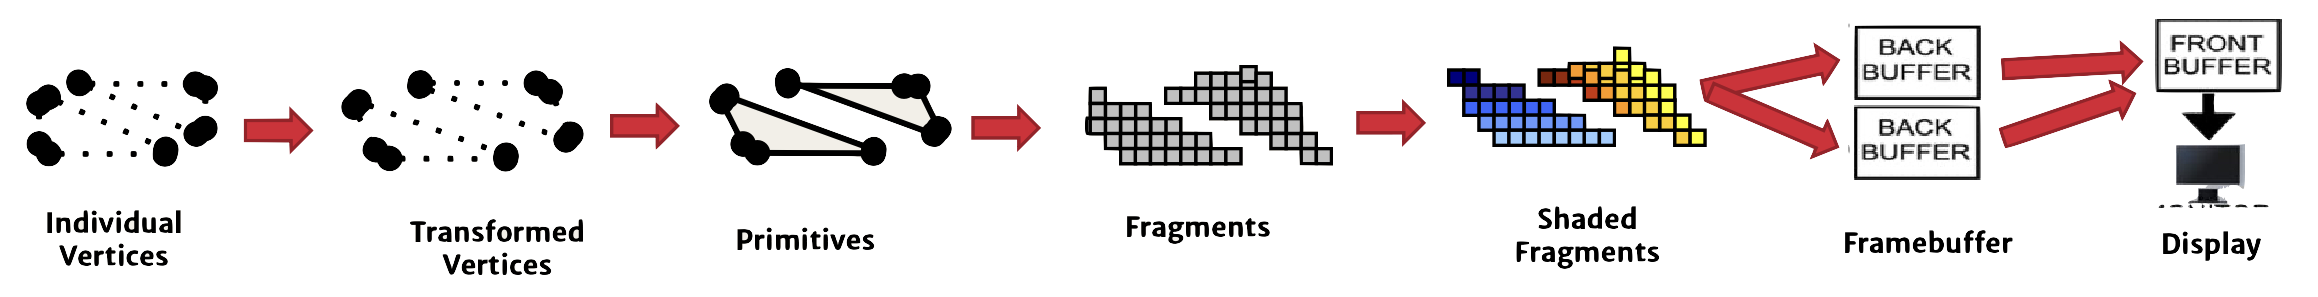
\includegraphics[width=\linewidth]{rasterization.png}
	\label{fig:rasterization}
\end{figure}
